\documentclass[kulak]{kulakarticle} % options: kulak (default) or kul
\usepackage{multicol}
\usepackage{caption}
\usepackage{subcaption}
\usepackage[spanish]{babel}

\title{Análisis de la investigación del Colegio de México}

\author{Dra. Daniela Aguirre Guerrero}
\date{Noviembre, 2022}
%\address{
	%\textbf{Groep Wetenschap \& Technologie Kulak} \\
	%Naam van de opleiding \\
	%Naam van het vak}

\begin{document}

\maketitle

\section{Metodología}
\subsection{Minería de datos}

\subsection{Análisis cuantitativo}

\subsection{Análisis de redes}

\subsubsection{Redes de co-autorías}

\subsubsection{Redes de co-ocurrencia de palabras clave}

\subsubsection{Métricas de centralidad}

\subsubsection{Detección de comunidades}


\section{Analisis cuantitativo}
\begin{table}[htbp]
	\centering
	\begin{tabular}{|l|l|}
		\hline
		\textbf{Description} & \textbf{Results} \\ \hline
		Timespan & 1964:2021 \\ \hline
		Sources (Journals, Books, etc) & 595 \\ \hline
		Annual Growth Rate \% & 8.94 \\ \hline
		Document Average Age & 8.99 \\ \hline
		Average citations per doc & 5.232 \\ \hline
		References & 43944 \\ \hline
		Documents & 1211 \\ \hline
		- article & 826 \\ \hline
		- book & 18 \\ \hline
		- book chapter & 143 \\ \hline
		- conference paper & 13 \\ \hline
		- editorial & 21 \\ \hline
		- letter & 2 \\ \hline
		- note & 16 \\ \hline
		- review & 171 \\ \hline
		- short survey & 1 \\ \hline
	\end{tabular}
	\caption{Resumen de los datos recolectados}
	\label{tb:resumen}
\end{table}




\begin{figure}[ht]

\centering
\begin{subfigure}[b]{0.48\textwidth}
\centering
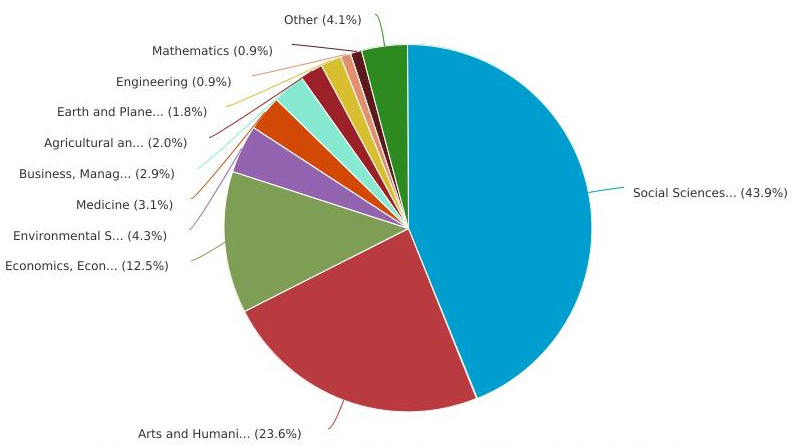
\includegraphics[width=1.1\textwidth]{imagenes/Scopus-Analyze-Subject.jpg}
\caption{Documentos por área de investigación}
\label{fig:docs_area}   
\end{subfigure}
\hfill
\begin{subfigure}[b]{0.48\textwidth}
\centering
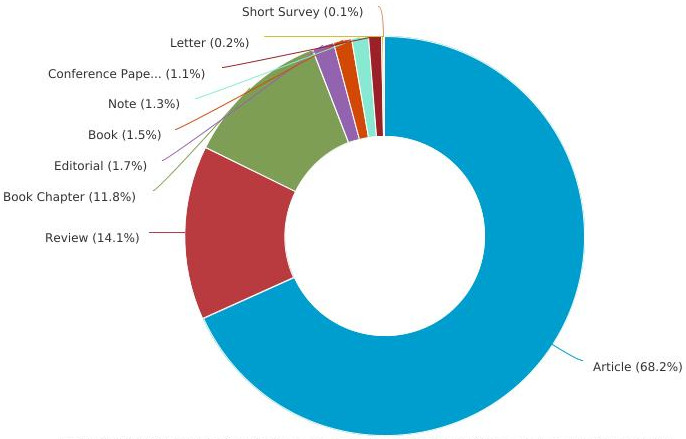
\includegraphics[width=0.95\textwidth]{imagenes/Scopus-Analyze-Doctype.jpg}
\caption{Documentos por tipo.}
\label{fig:docs_tipo} 
\end{subfigure}
\caption{Clasificación de los documentos analizados.}
\label{fig:docs_clasificacion} 
\end{figure}

\begin{figure}[ht]
	
	\centering
	\begin{subfigure}[b]{0.48\textwidth}
		\centering
		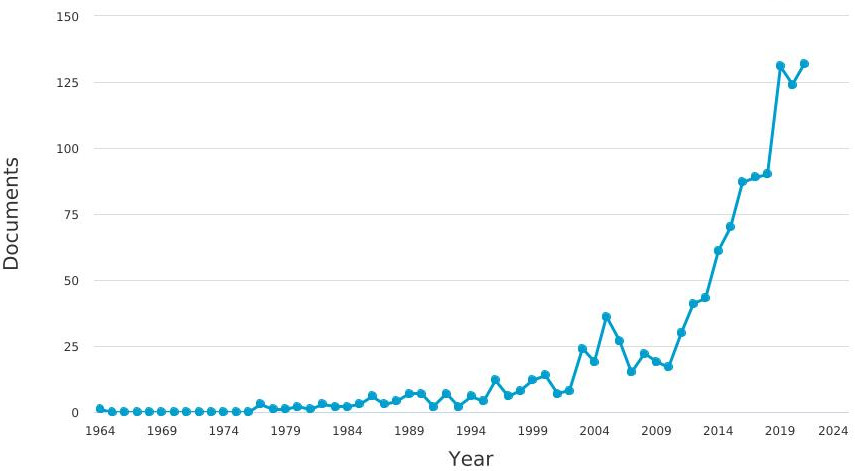
\includegraphics[width=1\textwidth]{imagenes/Scopus-Analyze-Year.jpg}
		\caption{Documentos publicados por año.}
		\label{fig:papers} 
	\end{subfigure}
	\hfill
	\begin{subfigure}[b]{0.48\textwidth}
		\centering
		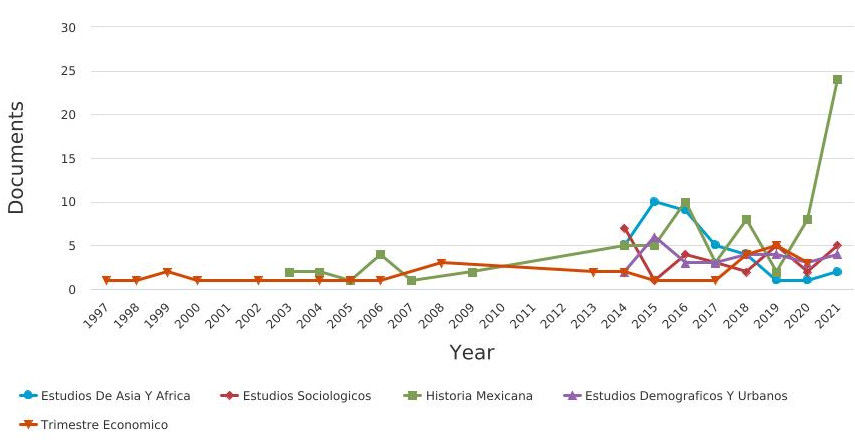
\includegraphics[width=1\textwidth]{imagenes/Scopus-Analyze-Source.jpg}
		\caption{Documentos publicados por año en las 5 fuentes más pupulares.}
		\label{fig:papers} 
	\end{subfigure}
	\caption{Evolución anual de las publicaciones.}
	\label{fig:docs_evolución} 
\end{figure}
\newpage
\section{Análisis de co-autorías}
\begin{table}[htbp]
	\centering
	\begin{tabular}{|l|l|}
		\hline
		\textbf{Description} & \textbf{Results} \\ \hline
		Authors & 1393 \\ \hline
		Authors of single-authored docs & 411 \\ \hline
		Single-authored docs & 703 \\ \hline
		Co-Authors per Doc & 1.88 \\ \hline
		International co-authorships \% & 20.48 \\ \hline
	\end{tabular}
	\caption{Información de co-autorías}
	\label{tb:resumen}
\end{table}

\begin{figure}[ht]
	\centering
	\begin{subfigure}[b]{0.48\textwidth}
		\centering
		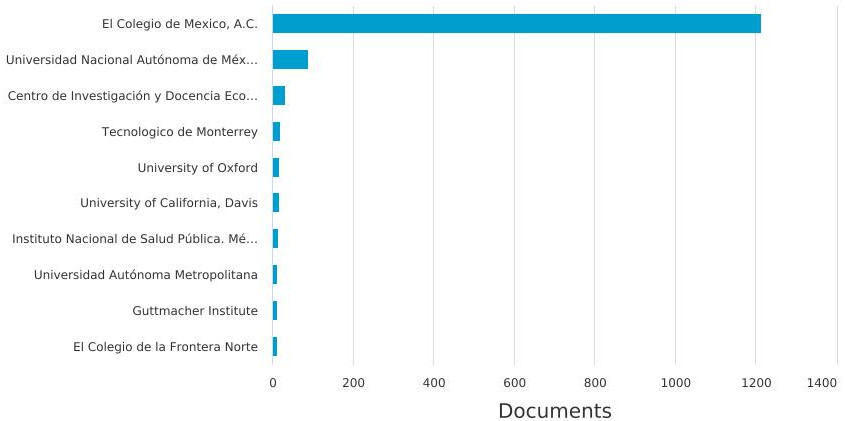
\includegraphics[width=\textwidth]{imagenes/Scopus-Analyze-Affiliation.jpg}
		\caption{Co-autorías por institución.}
		\label{fig:col_afiliacion}   
	\end{subfigure}
	\hfill
	\begin{subfigure}[b]{0.48\textwidth}
		\centering
		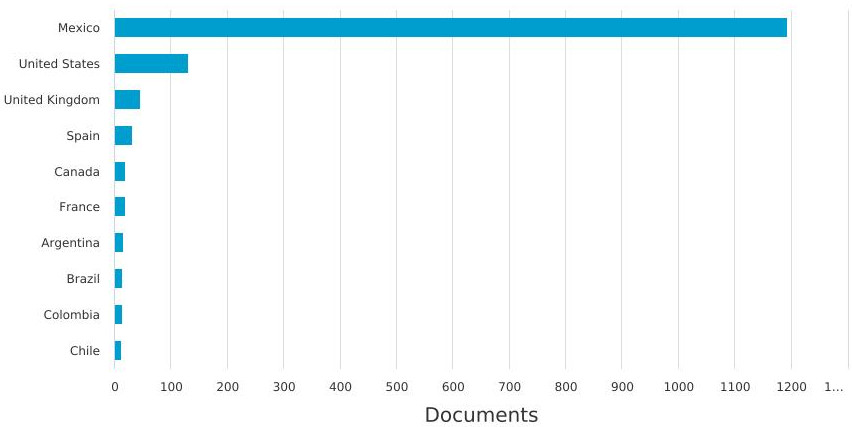
\includegraphics[width=\textwidth]{imagenes/Scopus-Analyze-Country.jpg}
		\caption{Co-autorías por país.}
		\label{fig:col_pais} 
	\end{subfigure}

	\caption{Distribución de las co-autorías.}
	\label{fig:docs_colaboraciones} 
\end{figure}

\newpage
\subsection{Redes de coautorías}
\begin{figure}[ht]

		\centering
		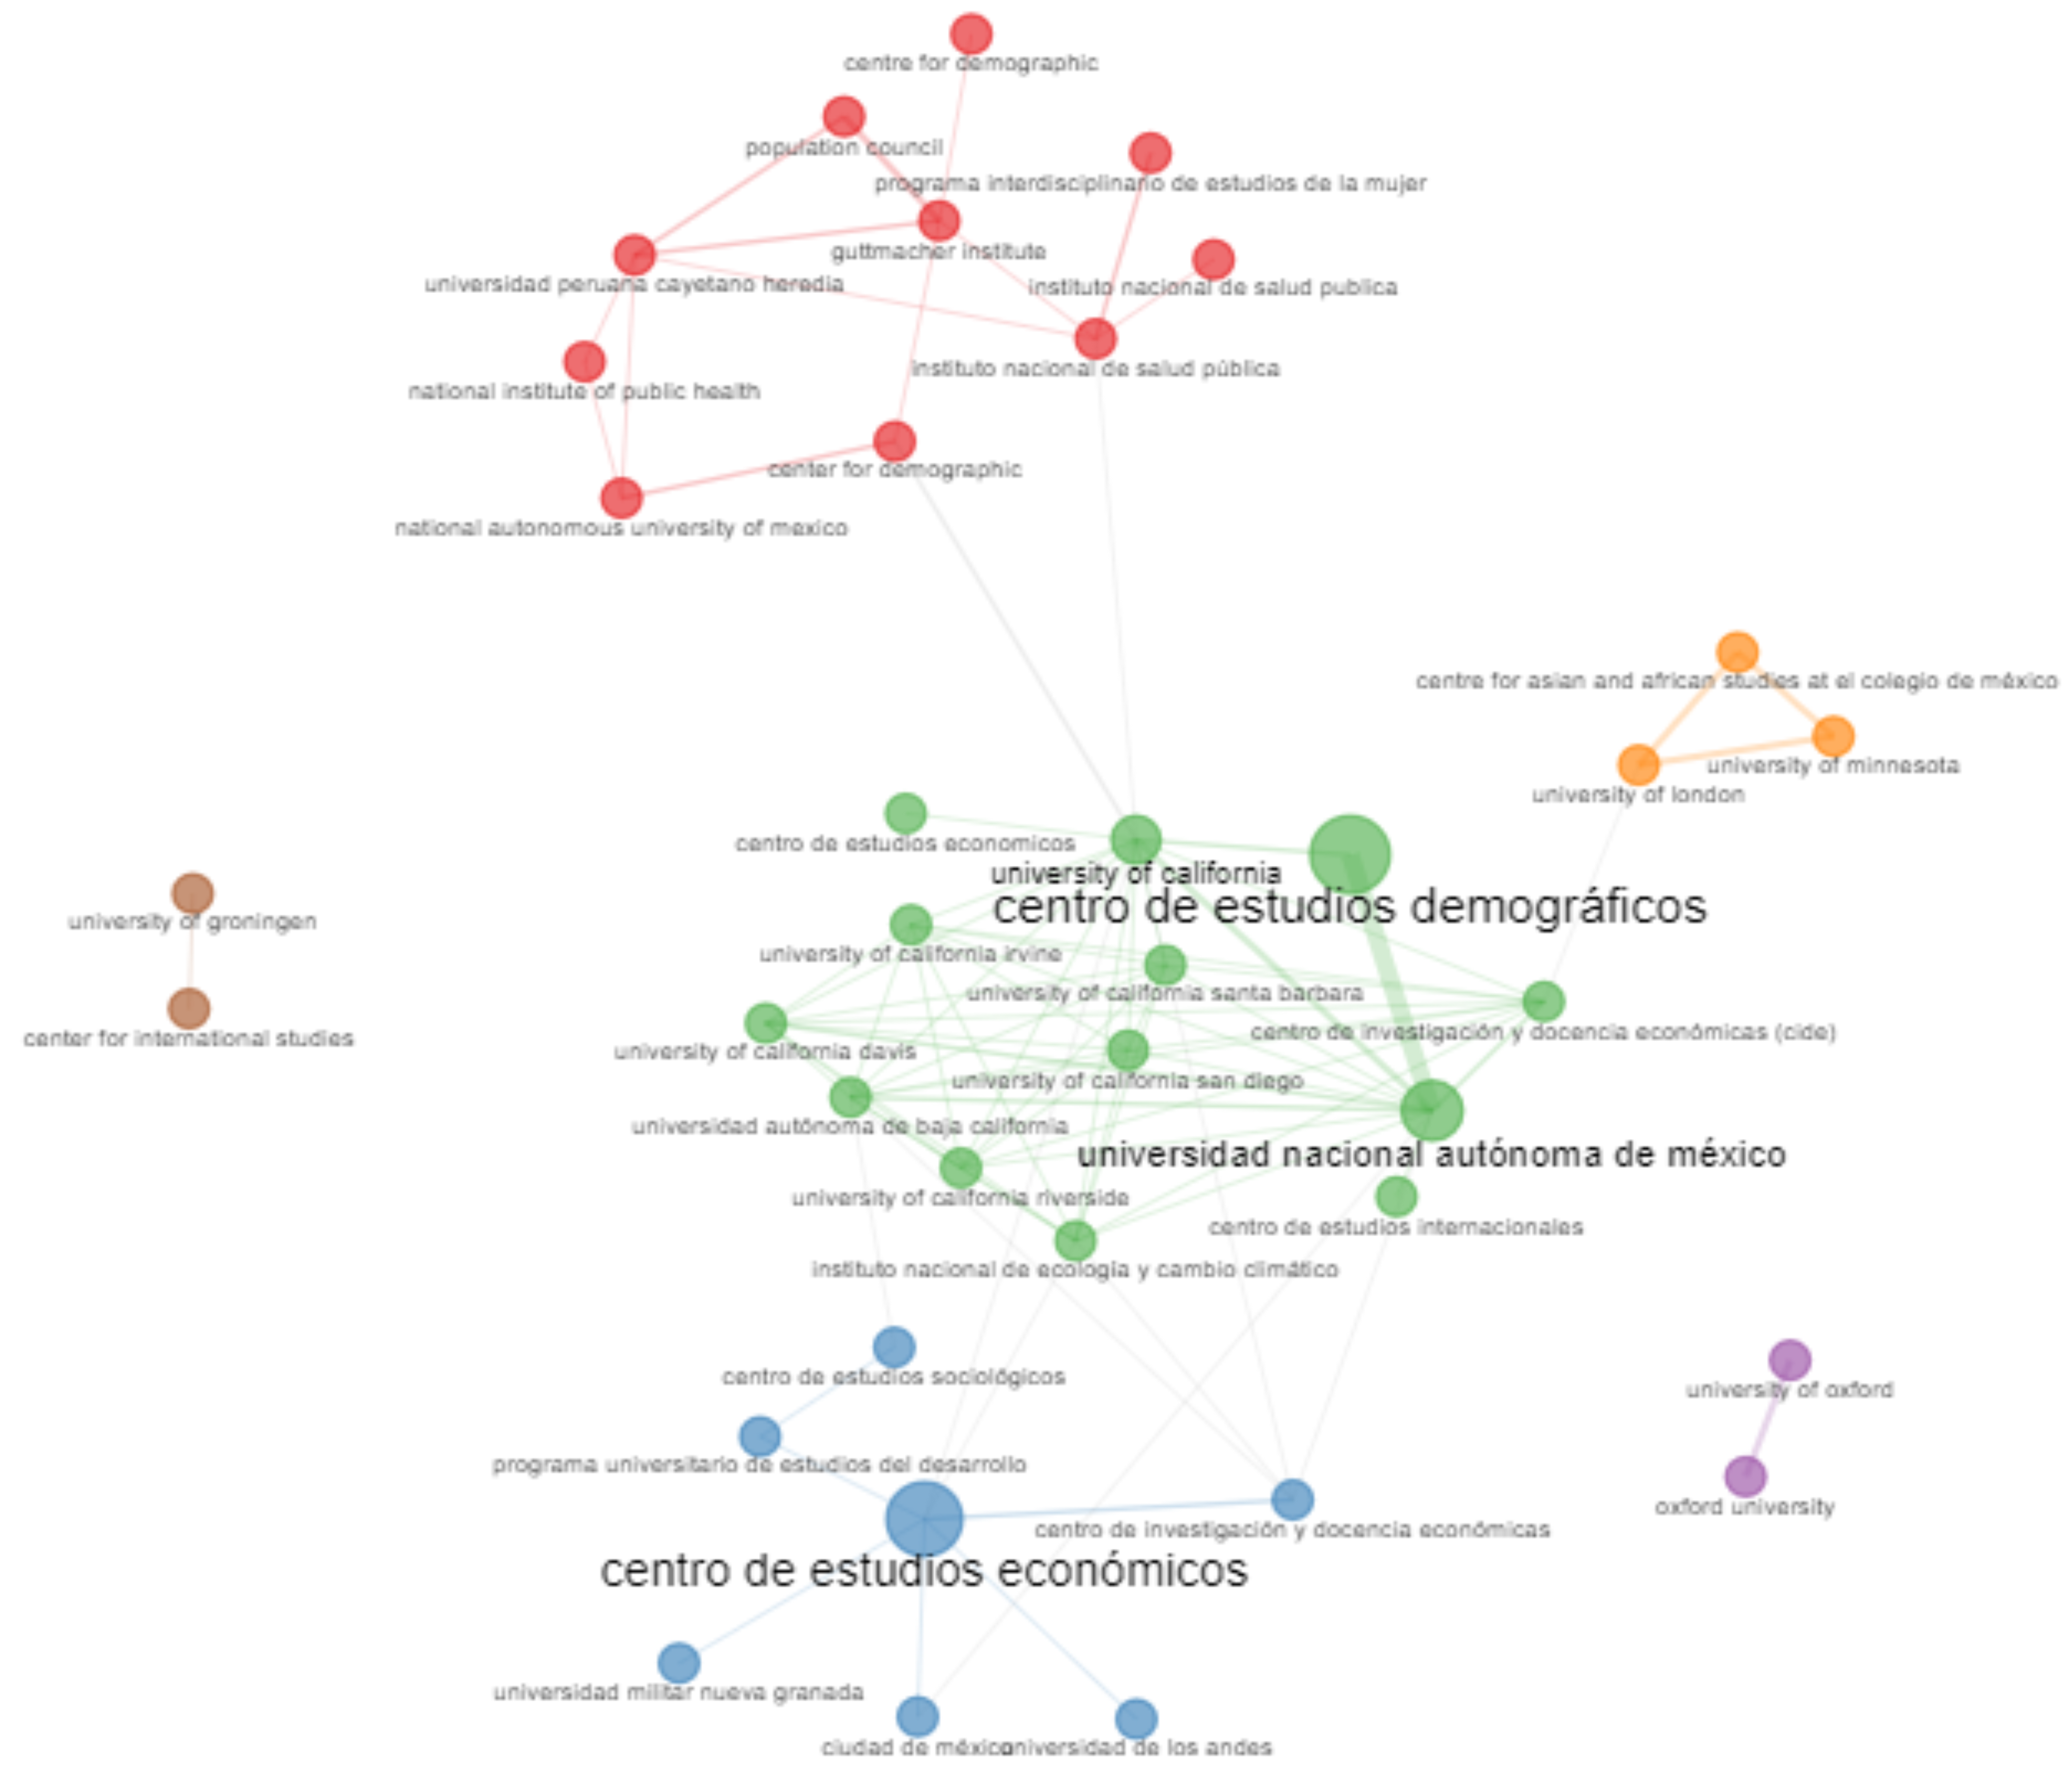
\includegraphics[width=0.8\textwidth]{imagenes/net_institucion.png}
		\caption{Red de co-autorías por institución.}
		\label{fig:net_afiliacion}   

\end{figure}

\begin{figure}[ht]
	\centering
	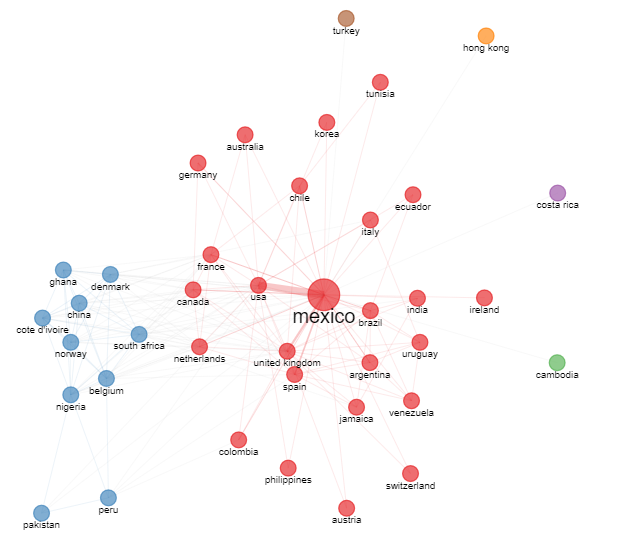
\includegraphics[width=0.8\textwidth]{imagenes/net_pais.png}
	\caption{Red de co-autorías por país.}
	\label{fig:net_country}   
	
\end{figure}



\section{Análisis conceptual}
\begin{table}[htbp]
	\centering
	\begin{tabular}{|l|l|}
		\hline
		\textbf{Description} & \textbf{Results} \\ \hline
		Keywords Plus & 1695 \\ \hline
		Author's Keywords & 2404 \\ \hline
	\end{tabular}
	\caption{Palabras clave contenidas en los documentos}
	\label{tb:keywords}
\end{table}



\begin{figure}[ht]
	\section{Autores con mayor H-Index y su relación con las tendencias de palabras clave y referencias}
	\centering
	\begin{subfigure}[b]{0.48\textwidth}
		\centering
		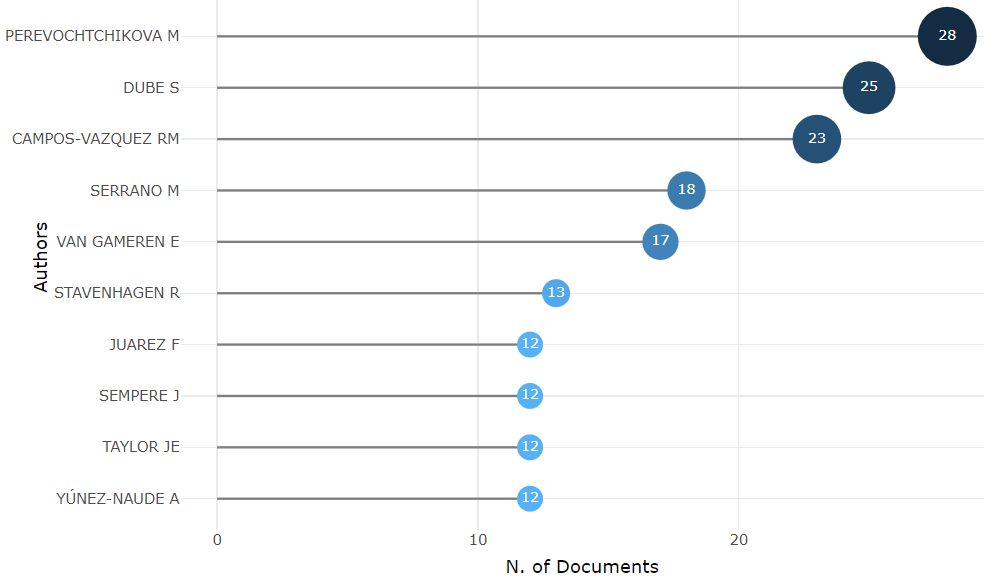
\includegraphics[width=.9\textwidth]{imagenes/au_productivos.png}
		\caption{Autores más productivos}
		\label{fig:au_productivos}   
	\end{subfigure}
	\hfill
	\begin{subfigure}[b]{0.48\textwidth}
		\centering
		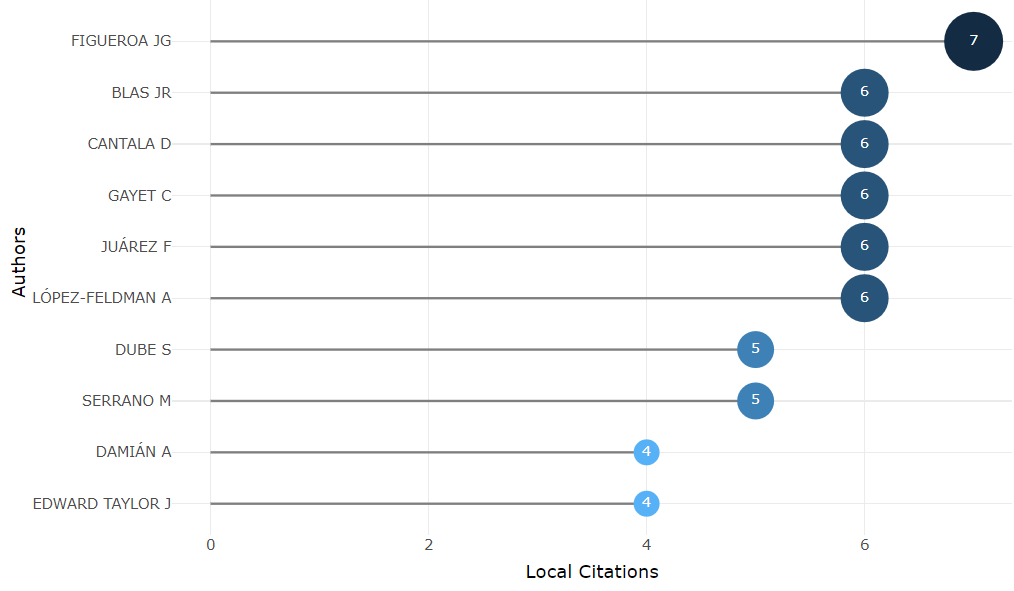
\includegraphics[width=0.9\textwidth]{imagenes/au_citados.png}
		\caption{Autores más citados (dentro del conjunto de datos análizado).}
		\label{fig:au_citados} 
	\end{subfigure}
	\caption{Autores más productivos y más citados.}
	\label{fig:autores} 
\end{figure}

\begin{figure}[ht]
	\centering
	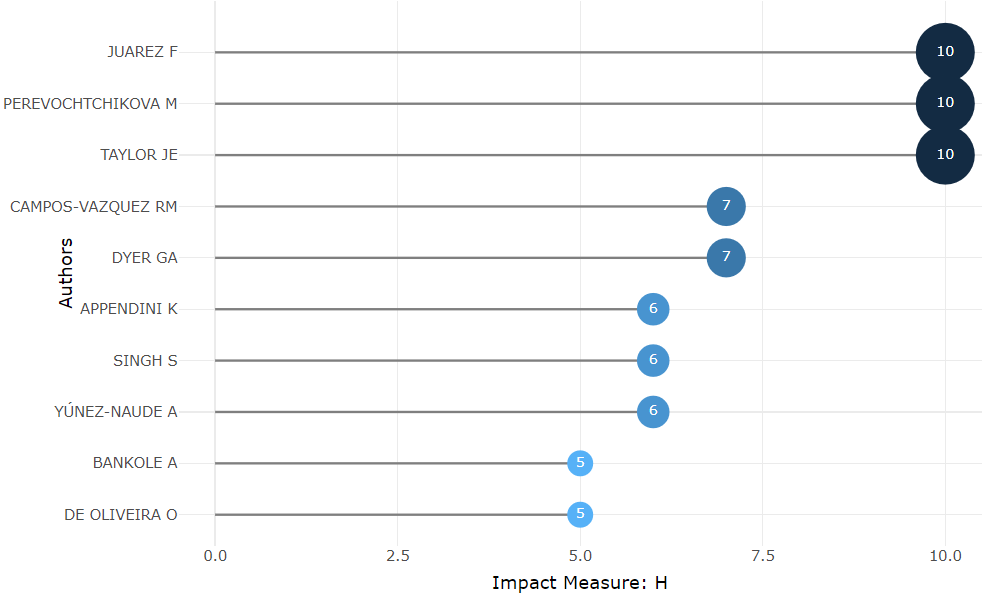
\includegraphics[width=0.8\textwidth]{imagenes/au_hindex.png}
	\caption{Autores con mayor \textit{H-Index} (dentro del conjunto de datos análizado).}
	\label{fig:au_hindex} 
\end{figure}

\begin{figure}[hp]

	\centering
	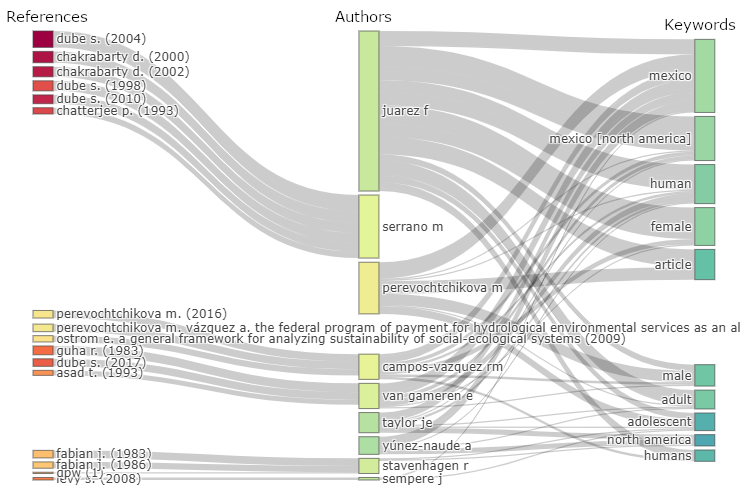
\includegraphics[width=0.8\textwidth]{imagenes/three_field.png}
	\caption{Impacto entre los autores con mayor \textit{H-Index} en las tendencias de referencias y palabras clave.}
	\label{fig:3field} 
\end{figure}

\begin{figure}[ht]
	
	\centering
	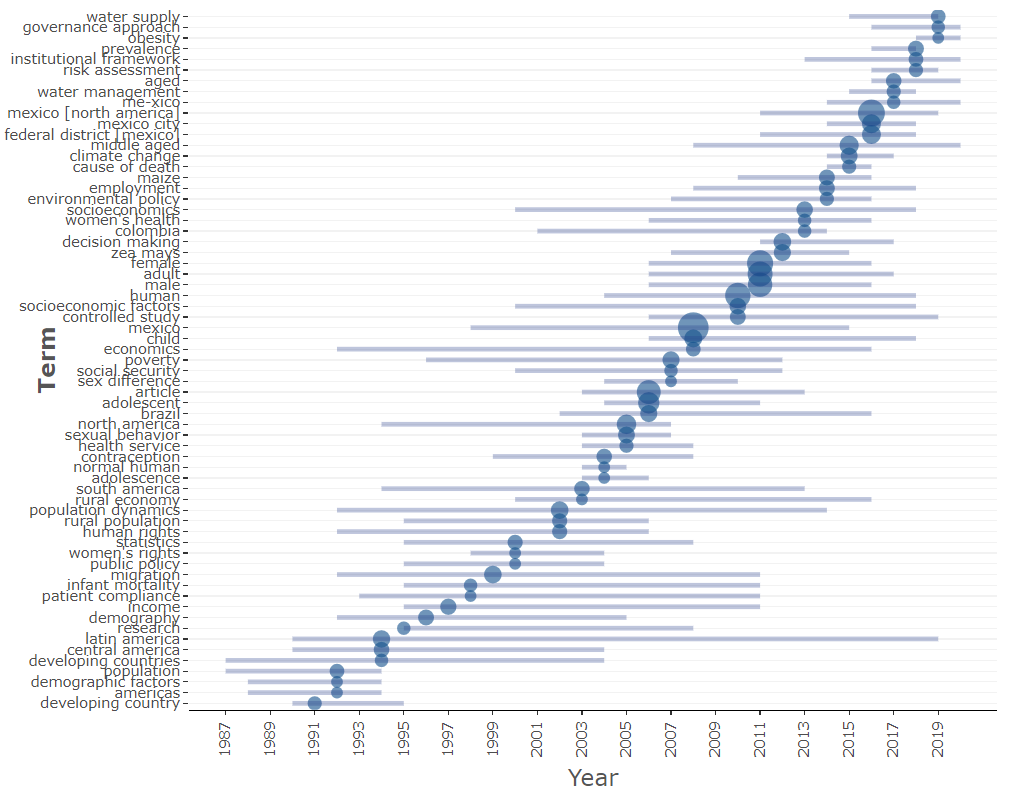
\includegraphics[width=0.8\textwidth]{imagenes/trend_topics.png}
	\caption{Evoluación de las temáticas de investigación con base en las tendencias en palabras clave.}
	\label{fig:trend_topic} 
\end{figure}





\end{document}
